\section{Quantiles Sketch}
\label{sec:quantiles}

\subsection{Overview}

Given a stream $A$ of items from an ordered domain, for every
$0< \phi < 1$, $\phi - quantile$ of $A$ is an item with rank 
$\lfloor \phi |A| \rfloor$, where the rank of item $i$ is the
number of elements in $A$ smaller than $i$.
An $\epsilon -approximate ~\phi - quantile$ is an element
with rank between $ (\phi - \epsilon) |A|$ and $ (\phi +
\epsilon) |A|$.
For every stream $A$, error $\epsilon$ and probabilty $\delta$,
a quantiles sketch algorithm produces a summary of $A$, which
supports $\epsilon -approximate ~\phi - quantile$ quires for
every $0< \phi < 1$ with probability
at least $1 - \delta$.

As in the Theta sketch presented in the previous section, there
is a tradeoff between summaries space cost and quires accuracy,
which have been widely studied in the past.
In this work we build on top of an algorithm presented
in~\cite{}, which storage cost grows logarithmically with the
input stream size.
Given a stream $A$, the storage cost of the algorithm is
$k*2^{log(\lfloor |A|/k \rfloor)}$, where $k = O((1/\epsilon)
\sqrt{log(1/\epsilon \delta)}$.
The main idea of the algorithm is a simple technique to
\emph{merge} two sets, $S_1$ and $S_2$ of $k$ items each, to a
single set $S$ of $k$ items:
First, set $S = S_1 \cup S_2$, and sort $S$. 
Then, with equal probability, retain either the even or the odd
items in the sorted order. 
This process is called \emph{zip}.


The algorithm maintains $\lfloor log(|A|/k) \rfloor$ weighted
levels, where each level is an array of size $k$ that either contains $k$ ordered
items or invalid (also called empty).
The weight of level $i$ is $2^{i-1}$.
In addition to the levels arrays, the algorithm uses a
\emph{bitPattern} variable that indicates what levels are valid,
and a \emph{base Buffer} of size $2k$, which is filled with items
from the stream.
Every time the baseBuffer is full, it is propagated (in place) to
the levels arrays in the following way:
First we use the bitPattern to find the first invalid level in
the levels array. 
We call this level the \emph{target} level, and at the end of
the propagation this level will become valid, while all the the
level beneath it will be invalid.
Next, we sort and zip the base buffer (with equal probability,
pick either the even or the odd items in the sorted order) into
the target level.
And then we repeat the following process from level $i=1$ to the
last level that precedes the target level:
Mergesort level $i$ with what is currently stored in the target
level into the base buffer, and then zip the base buffer into the
target level.
Finally, update the bitPatternt to indicate that all the target
level is now valid while all the level beneath are not.

Note that the wight of level $i+1$ is twice the wight of level
$i$ because it was zipped one more time, and thus it
``represents'' twice of the number of items ``represented'' in
level $i$.
This is important for quantiles accuracy.
In order to get a quantile we first have to build an
\emph{auxiliry} objects that contains two arrays:
(1) Sorted array of items, \emph{Iarr}, which 
contains all the items from all the valid levels, and (2) an
array of wights, called \emph{Warr}, that maps every item in
Iarr to its wight.
Then, to get the $~\phi - quantile$ of a stream $A$
we need to find the first index $ind$ in $Warr$ such that the
sum of all wights in $Warr$ till index $ind$ is $\lfloor \phi |A|
\rfloor$, and return $Iarr[ind]$.
Figue~\ref{fig:quantilesMerge} illustrates the algorithm.
Since it is not the focus of our paper we omit the error analysis
of the algorithm, and refer the interested reader to~\cite{} for
the proof and more details.

\begin{figure}[H]
    \centering
    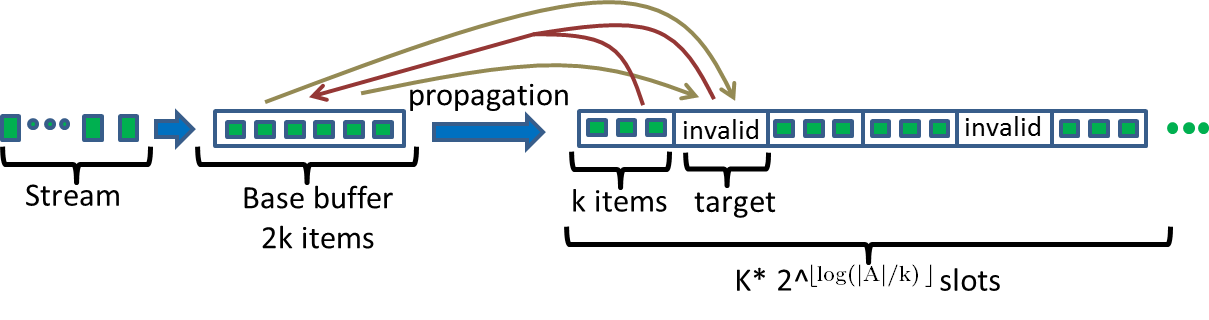
\includegraphics[width=5in]{images/quantilesPropogation.png}
    \caption{Quantile sketch. Propagation of the base buffer
    into the levels array.}
    \label{fig:quantilesMerge}
\end{figure}






\subsection{Concurrent algorithm}

Obviously protecting the sketch with a read/write lock yields
terrible performance. 
Not only that the fence decreases the throughput by a factor of 3
in update only scenario, but also since getting the quantiles
(reading) requires expensive computation, if we do it under lock
in mixed workload the throughput crashes.

Unfortunately, avoiding the lock is not an easy task. 
Since the propagation process (from the base buffer to levels
array), which requires most of the work in the algorithm, is
inherently very sequential, it cannot be done in parallel.
However, we can decrease the propagation rate without changing
the value of $k$. 
In other words, instead of propagating every $2k$ items we can
do it every $2^{i}k$, where $i \geq 0$ is a parameter that
impact accuracy (as described below).
This way we amortized the propagation cost and thus increase
throughput.

Our approach here is again to exploit locality and minimize
synchronization.
As in the concurrent Theta sketch, the idea is to have one
background thread and many worker threads.
Every worker thread maintains a local sketch with bounded number
of levels, and every time the local sketch fulfils, it passes
its last level to the background thread to propagate it to the
shared sketch.
In order to reduce the number of propagated items to $k$, we
propagate when the last level of the local sketch is the only
valid level.
For a sketch with $i$ local levels, it happens every $2^ik$
items from the stream.
%Note also that if a thread have $i$ local levels, it passes $k$
%items to the background thread every $2^ik$ items from the
% stream.
The optimal number of local levels depends on the number of
concurrent worker threads.
Since we have only one background thread, the propagation
throughput is constant.
Meaning that when we have more worker threads, each thread gets
less help from the background thread, and thus
we need to make sure each thread needs the background thread
less often.
Therefore, for perfect scalability we increase the number of
local levels with the number of worker threads.

After asking the background thread to propagate its last level,
a worker thread starts filling its local sketch again, hoping the
propagation process will complete faster.
As in the Theta sketch, the synchronization between the
background thread and a worker thread $t_i$ is done over a
single atomic variable $P_i$.

To propagate level $i$ from a local sketch to the shared sketch,
the background thread uses the mechanism described in the
sequential quantiles sketch overview above with the following
change:
Instead of starting from zipping the base buffer
into the target level, it starts from level $i$.
If level $i$ in the shared sketch is valid, the background
thread merges it (via merge sort) with the local level $i$ into
the base buffer, and continue the propagation to the next level
as before.
Otherwise, it simple copy the local level $i$ to the shared level
$i$.
The target buffer in this case is the first invalid level that is
not smaller than $i$.
Figure~\ref{cocurrentQuntiles} illustrates the concurrent
quantiles sketch architecture.

Recall that in order to read (getQuantiles), readers build an
auxiliary object based on the levels array and the bitPattern
that describes it.
Therefore, in order to be able to read concurrently with
background propagation, a reader must obtain a snapshot of the
levels array.
We solve it with the double successful collect technique.
First, we define the bitPatern to be atomic in order to make sure
that a propagation is visible to all readers after the
bitPattern is updated.
Second, a reader repeatedly tries to obtain a consistent view of
the levels array: it reads the bitPattern, then the levels array,
and then the bitPattern again.
If the bit pattern did not change between the two reads, the
reader has a consistent view.
Otherwise, it tries again.

Recall that during the propagation process, the background
thread may read many levels, but writes only to the target level,
which is invalid at this point.
Therefore, a reader can be sure that the valid levels it reads
between the two identical reads of the bitPatern are consistent
even though the background thread concurrently
propagating.
In addition, note that a reader do not have to read all the valid
levels each time it fails to obtain a successful double collect.
Since a valid level may become invalid and then valid again
(with different items) only after a higher invalid level become
valid, if two sequential reads of the bitPatern has a
common suffix, the reader must read only the valid levels in
the different prefix of the later bitPattern read. 
It is guaranteed that the valid levels in the suffix are
unchanged.

Note that obviously the reads are not wait-free since the
bitPatern can potently be changed faster than the readers ability
to read.
However, note that the propagation time (and thus
the time between bitPattern changes) is longer when the target
level is higher, and once in a while the background thread must
propagate to high levels.
So, eventually the propagation will be long enough for
all the reader to obtain a snapshot of the levels array. 
However practically, we see that the readers are able to do it
much faster, and the snapshot time is negligible to the time to
build the auxiliary object.

\begin{algorithm}[tb]
\small
%\begin{multicols}{2}
\begin{algorithmic}[1]

%\State {\bf Sketch variables:}
\Vars
\State \emph{sampleSet}, init $[ ]$ \Comment global samples
\State \emph{maxLevel} \Comment global max level
\State \emph{bitPattern}, init 0 \Comment bit array of valid levels
\State 
\Statex
\ForEach{update thread $t_i$}
	\State \emph{baseBuffer$_i$}, init $[ ]$ \Comment local array
	\State \emph{buf$_i$}, init $[ ]$ \Comment local sample set
	\State \emph{aux$_i$}, init $[ ]$ \Comment auxiliary array
	\State {\tt atomic} $P_i$, init $1$ \Comment for synchronization
\EndFor
\EndFor

\Statex
\Procedure{query}{$\phi$}
\State \emph{old} $\leftarrow$ \emph{0}
\State \emph{new} $\leftarrow$ \emph{bitPattern}
\While{\emph{new} $\neq$ \emph{old}}
	\State \emph{highestDiff} $\leftarrow$ rightmost 1 bit in \emph{new} that is 0 in \emph{old}
	\ForAll{\emph{lvl} s.t. bit \emph{lvl} is 1 in \emph{new} and \emph{lvl} $\leq$ \emph{highestDiff}}
		\If{bit \emph{lvl} is 0 in \emph{old}}
			\State \emph{localSampleSet[lvl]} $\leftarrow$ \emph{sampleSet[lvl]}
		\EndIf
	\EndFor
	\State \emph{old} $\leftarrow$ \emph{new}
	\State \emph{new} $\leftarrow$ \emph{bitPattern}
\EndWhile

\ForAll{\emph{lvl} s.t. bit \emph{lvl} is 1 in \emph{new}} \label{l:caught-snapshot}
	\ForAll{\emph{sample} in \emph{localSampleSet[lvl]}}
		\State append $\langle$\emph{sample},\emph{$2^{lvl}$}$\rangle$ to \emph{tuples}
	\EndFor
\EndFor
\State sort $tuples$ by $sample$
\State $pos \leftarrow \min {\{\lfloor N \times \phi \rfloor, N-1\}}$
\State $sum \leftarrow 0$
\State $ind \leftarrow 0$
\While{$sum \leq pos$}
	\State $sum \leftarrow sum + tuples[ind].weight$
	\State $ind \leftarrow ind + 1$
\EndWhile
\State \Return $tuples[ind-1].sample$ 
\EndProcedure
%\Statex

\Procedure{update$_i$}{$val$}
\State ordered insert $val$ into $baseBuffer_i$
\If{num items in $baseBuffer_i$ = $2k$}
	\State $tmpK \leftarrow zip baseBuffer$
	\State $target \leftarrow$ \Call {propogate}{$tmpK$, $buf_i$, $bitPattern_i$}
	\If{$target$ equals $maxLevel$}
		\State wait until $P_i>0$
		\State $aux_i \leftarrow buf_i[maxLevel]$
		\State set bit $maxLevel$ in $bitPattern_i$ to 0
		\State $P_i \leftarrow$ 0
	\EndIf
\EndIf
\EndProcedure

\Procedure{propagator}{}
\While {true}
\ForAll{update thread $t_i$ s.t. $P_i =0$}
		\State $tmpK \leftarrow aux_i$
		\State $P_i \leftarrow 1$
		\State \Call{propogate}{$tmpK$,$sampleSet$,$bitPattern$}
		\State $N \leftarrow N + K \times 2^{maxLevel}$
\EndFor
\EndWhile
\EndProcedure

\Procedure{propagate}{\emph{tmpK}, \emph{buf}, \emph{bitPattern}}
% There is a bug here. The bitPattern must change atomically all it's bits.
\State \emph{target} $\leftarrow$ leftmost zero bit in \emph{bitPattern} after \emph{maxLevel}
\State \emph{bitPatternMask} $\leftarrow$ 0
\For{$lvl \in \{1,\dots,target-1\}$}
		\State \emph{tmp2K} $\leftarrow$ mergeSort of \emph{tmpK} with \emph{buf[i]}
		\State \emph{tmpK} $\leftarrow$ zip \emph{tmp2K} \label{l:zip}
		\State set bit \emph{lvl} in \emph{bitPatternMask} to 1
\EndFor
\State \emph{buf[target]} $\leftarrow$ \emph{tmpk}
\State set bit \emph{target} in \emph{bitPatternMask} to 1
\State \emph{bitPattern} $\Leftarrow$ \emph{bitPattern} $\oplus$ \emph{bitPatternMask}
\State \Return \emph{target}
\EndProcedure

\end{algorithmic}
%\end{multicols}
\caption{Concurrent Quantiles sketch algorithm.}
\label{alg:concurrent-theta}
\end{algorithm}


\begin{figure}[H]
    \centering
    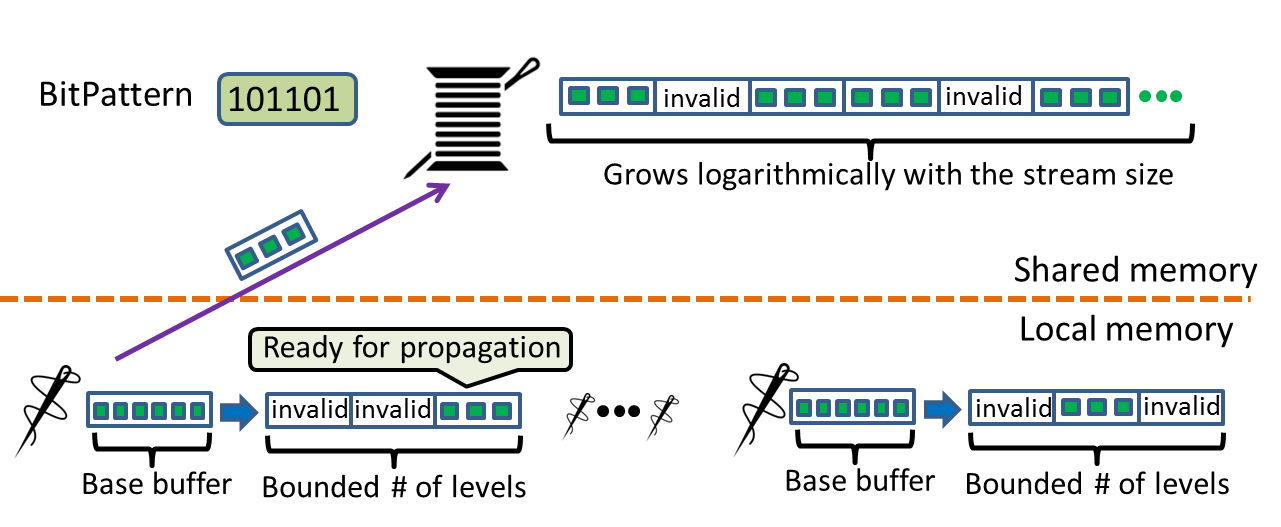
\includegraphics[width=5in]{images/cocurrentQuntiles.png}
    \caption{Concurrent Quantiles sketch architecture.}
    \label{cocurrentQuntiles}
\end{figure}


\subsection{Analysis}
In order to capture the randmoness of the zip operation, we will model the values provided in the stream
as arriving in tuple form $\langle$\emph{val},\emph{C}$\rangle$, where $C\in\{0,1\}$, the that values of
\emph{C} provided externally. The zip operation performs $C_1 \oplus C_2 \oplus \dots \oplus C_{2K}$, and if
the answer is 0 then the operation chooses the even places in the set, if 1 then the odd places. We denote
by $A_S^D$ the histories of the deterministic algorithm, and by $A_S^r$ its r-relaxation. Finally we denote
$A_C$ our concurrent algorithm.
When $A_C$ uses \emph{N} update threads, its relaxation is $r=2NK2^{maxLevel}$. We 
will show that $A_C$ is stronly linearizabile with respect to the relaxed specification $A_S^r$.

\subsubsection{Strong linearizabilty wrt relaxed semantics}
To prove correctness, we will first prove that the deterministic concurrent algorithm behaves in the same way
as the sequential deterministic algorithm.

\begin{claim}
	Each update thread upholds $A_S^D$.
\end{claim}

\begin{proof}
This is true by definition, as this is the algorithm the update threads are running.
\end{proof}

\begin{claim} \label{quantiles-propogator-proof}
	The propagator behaves like $A_S^D$.
\end{claim}

\begin{proof}
	When an update thread propogates it's \emph{buf}, we can look at the algorithm as if all the updates
	that the update thread executed happened now to the propgator, in the order they happened in the update thread.
	Therefore the propogator will make the same zip choices, and therefore behaves like $A_S^D$.
\end{proof}

As opposed to Theta, here we have update(v) that can be \emph{reflected} by other updates. We define reflection
by having the value either included or not included in the zipped set. Performing a zip 
{$v_1$, $\dots$,$v_{2K}$}, and assuming the even indexes were chosen,
 we say that for any i, $v_i$ is reflected in  {$v_2$, $v_4$, $\dots$,$v_{K_K}$}.

\begin{invariant}
	Consider a finite execution $\sigma$ of  $A_c$ and an update(v) that returns in $\sigma$. 
Then at the end of $\sigma$, the updated is reflected in 
$\bigcup_{i=1}^N (\mathit{buf_i} \cup \mathit{aux_i}) \; \cup$ \emph{sampleSet}
\end{invariant}

\begin{proof}
	The proof is by induction on the length of $\sigma$. The base for the empty execution is immediate. 
	Now consider execution steps that can change the invariant.
	First, consider an update that does not cause \emph{baseBuffer}$_i$ to fill up, in this case $v \in baseBuffer_i$.
	Next, if the update fills ups \emph{baseBuffer}$_i$ but doesn't trigger  propogate, then the value is reflected
	in \emph{buf}$_i$.
	Next, consider the propagation. according to \ref{quantiles-propogator-proof} the value being zipped in
	the update threads is equivelant to updating the propogator thread directly, therefore the update will be
	reflected in $sampleSet$.
\end{proof}

We point out that according to \ref{quantiles-propogator-proof} there is no difference between the update
threads performing zip and passing the zipped values up to the propogator, or the propogator doing the all work.

% f is like before and this should probably be said
As in the proof for the Theta sketch, our storng linearizabilty proof uses two mappings, \emph{f} and \emph{g},
from executions of $A_C$ to sequential executions. For an execution $\sigma$ of $A_C$, $f(\sigma)$ is the sequential
execution of $A_S$ consisting of operations invoked in $\sigma$, ordered according to their invokation context. By
definition $f(\sigma)$ preserves real-time order of $\sigma$ and is prefix preserving. To prove strong linearizabilty
wrt to relaxed semantics, it remains to show that $f(\sigma)$ $\in$ $A_S^r$.
We define our second mapping, \emph{g}, by ordering the operations to visibilty points.
\begin{itemize}
	\item
	Visibility points of queries are when the thread captures a snapshot, i.e on line \ref{l:caught-snapshot}.
	%same as their linearization points. 
	\item
	For an update$_i$($v$) in $\sigma$, let \emph{t} be the next time in $\sigma$ where threat $i$ propogates
	$buf_i$ to $aux_i$. The updates visibilty point is the update of \emph{bitPattern} by the propogator thread
	after time \emph{t}.
	%the call to propogate by the propogator 
	\end{itemize}

As with Theta, we will show that for every execution $\sigma$ of $A_c$:
(1) ${\cal H}(g(\sigma)) \in A^D_s$, and 
(2)  ${\cal H}(f(\sigma))$ is a $2NK2^{maxLevel}$-relaxation of ${\cal H}(g(\sigma))$.  
Together, this will imply that ${\cal H}(f(\sigma)) \in A^{r}_s$, as needed.

In \ref{quantiles-propogator-proof} we have already shown (1).
To prove (2), observe first that since an operation's invocation is always at or before its 
visibility point, $g(\sigma)$ includes a subset of the operations in $f(\sigma)$. 
It remains to show  that every operation invocation in $g(\sigma)$ is preceded by all 
but at most $2NK2^{maxLevel}$  of the invocations that precede the same operation in $f(\sigma)$. 
To prove this, we show that for every prefix $\sigma'$ of $\sigma$, $g(\sigma')$ includes all 
but at most $2NK2^{maxLevel}$  of the invocations in $f(\sigma')$.
Observe that 
every operation in $f(\sigma')$ that is not included in $g(\sigma')$ is update$_i$($v$) such that $v$
was  retained in \emph{buf$_i$} and did not yet propagate to sampleSet at the end of $\sigma'$. 
In this case, the update is reflected either in \emph{buf$_i$} or in  \emph{aux$_i$}, each of which 
includes at most $K2^{maxLevel}$ samples, and since there are $N$ update threads, there are at most
$2NK2^{maxLevel}$ such values, as needed.


We have proven the following:

\begin{lemma}%[Strong linearizability] 
$A_c$  with $N$ update threads is strongly linearizable wrt $A^{2Nb}_s$.
\label{lemma:quantiles-strong}
\end{lemma}


TODO: Prove strong linearizabilty.

We allow reader to skip local sketches

The number of local levels vs accuracy 
